\documentclass[accentcolor=tud6b,colorbacktitle,inverttitle,landscape,german,presentation,t]{tudbeamer}
\usepackage{ngerman}
\usepackage[utf8]{inputenc}
\usepackage{graphicx}
\usepackage{multirow}
\providecommand\thispdfpagelabel[1]{}

\begin{document}

\title[MLDM: Projekt Aufg 4-6]{Maschinelles Lernen Symbolische Ansätze:\\ Projekt Aufgaben 4-6}
\subtitle{}

\author[brehmer\_endreß\_fahrer]{Joachim Brehmer, Jeannine Endreß, Uli Fahrer}
%\institute[]{}

\date{\today}

\begin{titleframe}
\tableofcontents
\end{titleframe}

    \section{Aufgabe 4 - Entscheidungsbäume}
    
    \subsection{Benutzte Datensätze}
    
    \begin{frame}[t]
    \frametitle{Aufgabe 4 - Entscheidungsbäume\\ Benutzte Datensätze}
        \begin{itemize}
            \item Breast Cancer Data
            \item 1984 United States Congressional Voting Records Database
        \end{itemize}
        \vfill
        $\rightarrow$ Auf beide Datensätze unsupervised Filter ``ReplaceMissingValues'' auf unvollständige Attribute anwenden\\
        $\rightarrow$ Danach Lernen mit ID3 und J48 und Vergleich der Ergebnisse
    \end{frame}
    
    \subsection{ROC Kurven}
    
    \begin{frame}[t]
    \frametitle{Aufgabe 4 - Entscheidungsbäume\\ ROC Kurven}
        \begin{figure}[htbp]
            \centering
            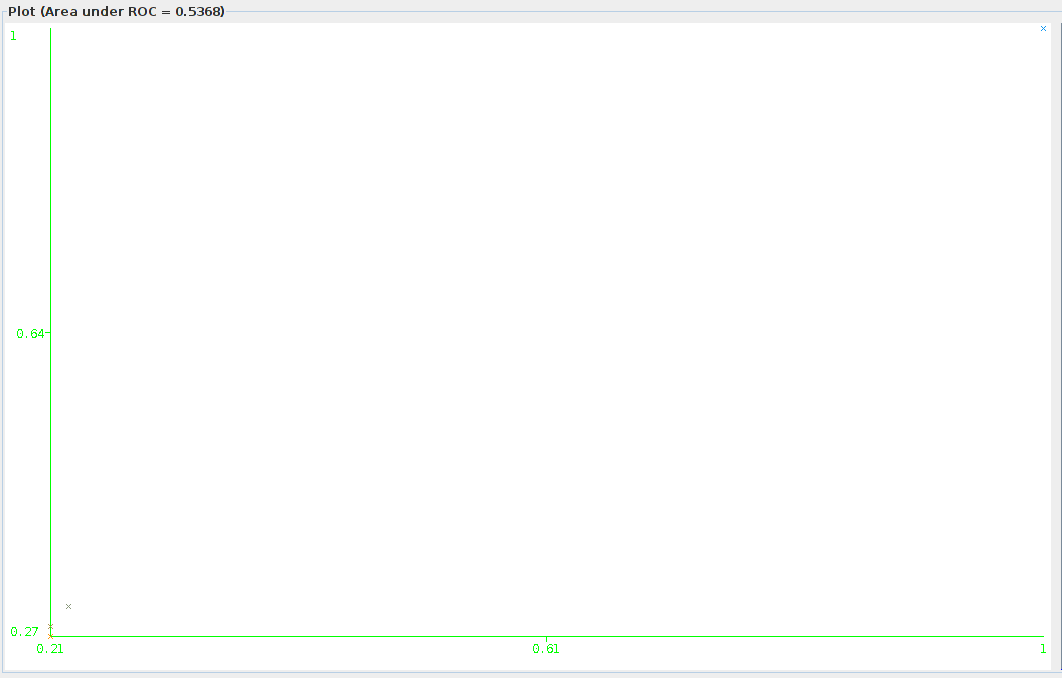
\includegraphics[height=5cm]{breastcancer-id3}
            \caption{ID3 - ROC-Kurve für ``breast-cancer''}
        \end{figure}
    \end{frame}
    
    \begin{frame}[t]
    \frametitle{Aufgabe 4 - Entscheidungsbäume\\ ROC Kurven}
        \begin{figure}[htbp]
            \centering
            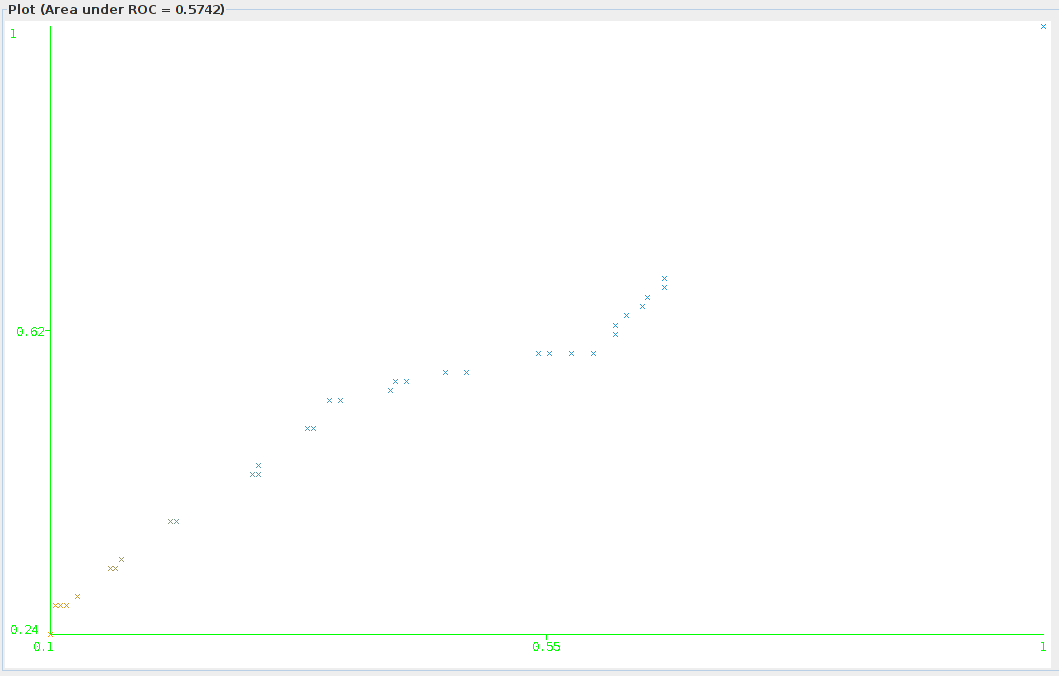
\includegraphics[height=5cm]{breastcancer-j48-unpruned}
            \caption{J48 (unpruned) - ROC-Kurve für ``breast-cancer''}
        \end{figure}
    \end{frame}
    
    \begin{frame}[t]
    \frametitle{Aufgabe 4 - Entscheidungsbäume\\ ROC Kurven}
        \begin{figure}[htbp]
            \centering
            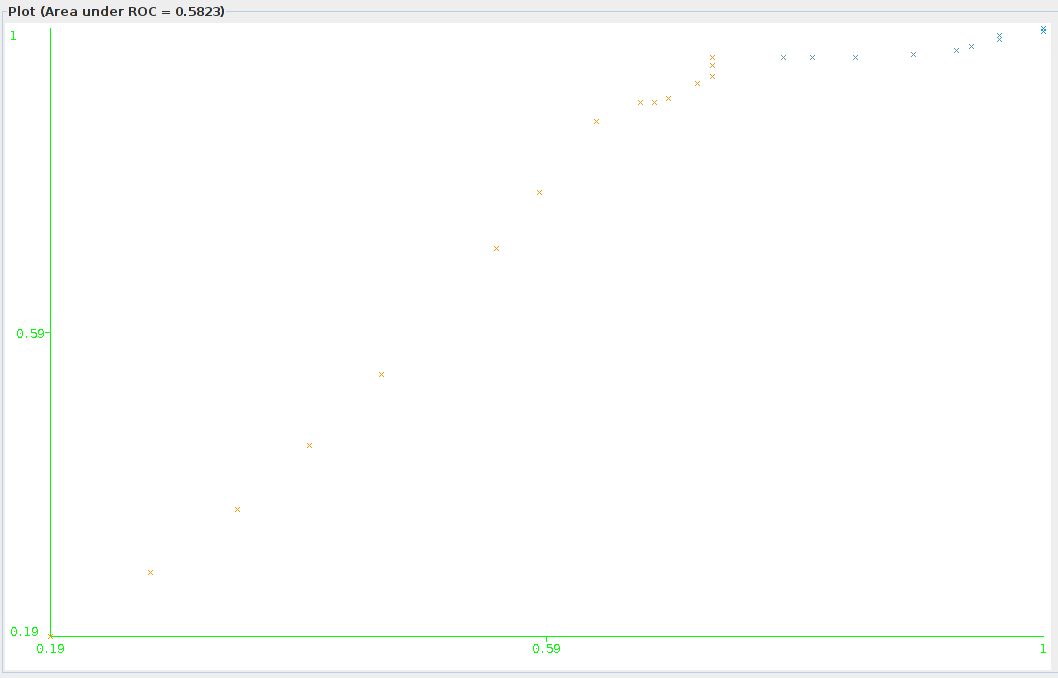
\includegraphics[height=5cm]{breastcancer-j48-pruned}
            \caption{J48 (pruned) - ROC-Kurve für ``breast-cancer''}
        \end{figure}
    \end{frame}
    
    \begin{frame}[t]
    \frametitle{Aufgabe 4 - Entscheidungsbäume\\ ROC Kurven}
        \begin{figure}[htbp]
            \centering
            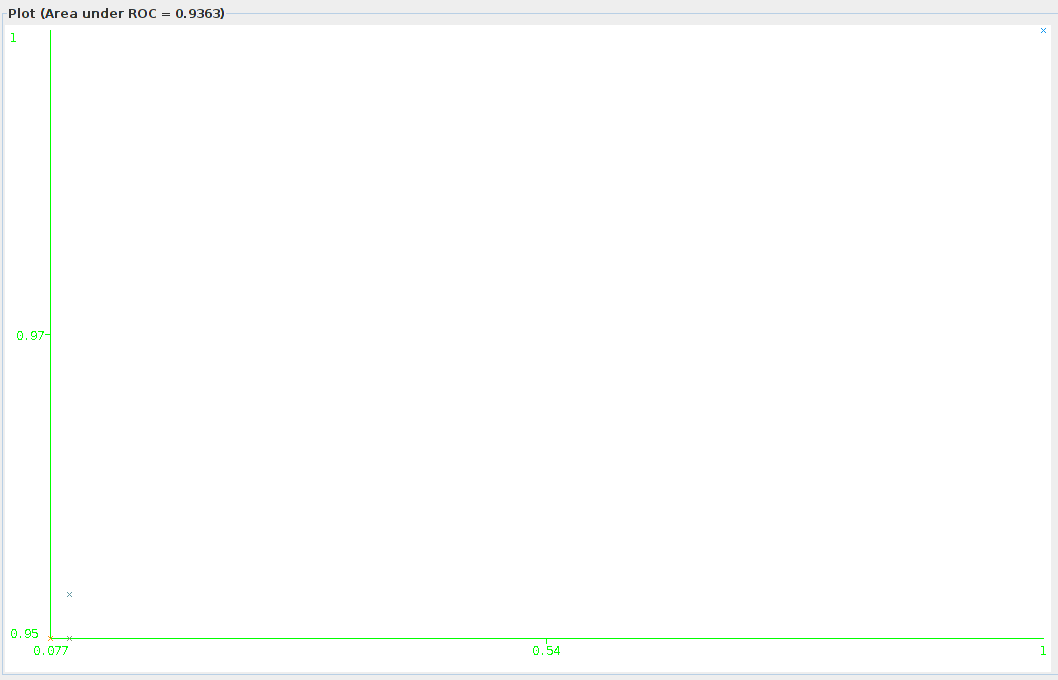
\includegraphics[height=5cm]{vote-id3}
            \caption{ID3 - ROC-Kurve für ``vote''}
        \end{figure}
    \end{frame}
    
    \begin{frame}[t]
    \frametitle{Aufgabe 4 - Entscheidungsbäume\\ ROC Kurven}
        \begin{figure}[htbp]
            \centering
            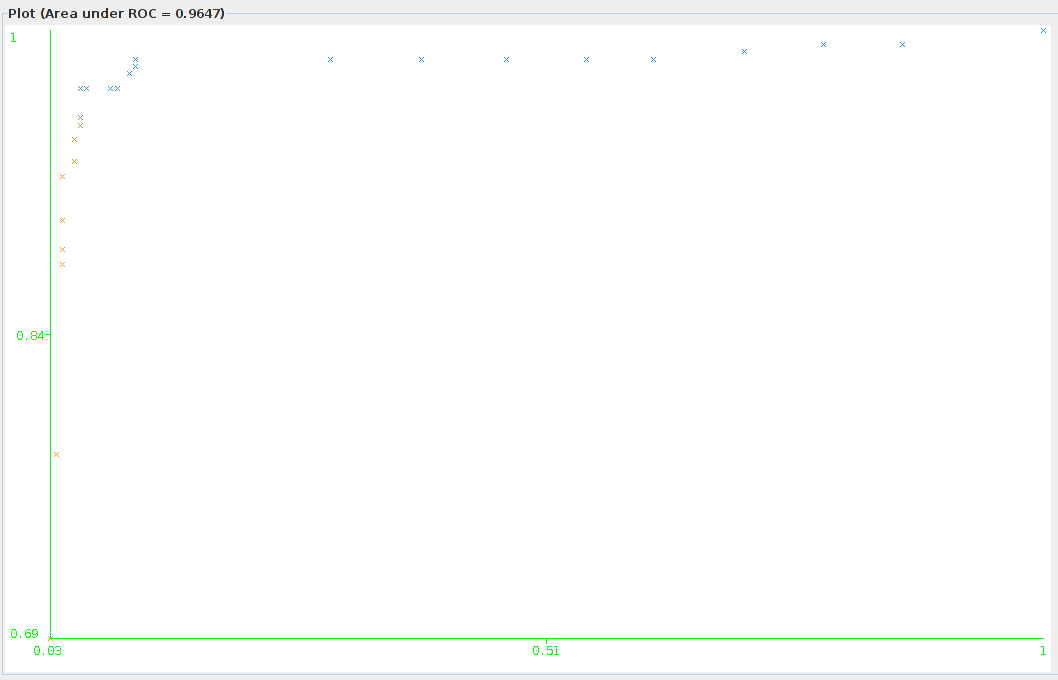
\includegraphics[height=5cm]{vote-j48-unpruned}
            \caption{J48 (unpruned) - ROC-Kurve für ``vote''}
        \end{figure}
    \end{frame}
    
    \begin{frame}[t]
    \frametitle{Aufgabe 4 - Entscheidungsbäume\\ ROC Kurven}
        \begin{figure}[htbp]
            \centering
            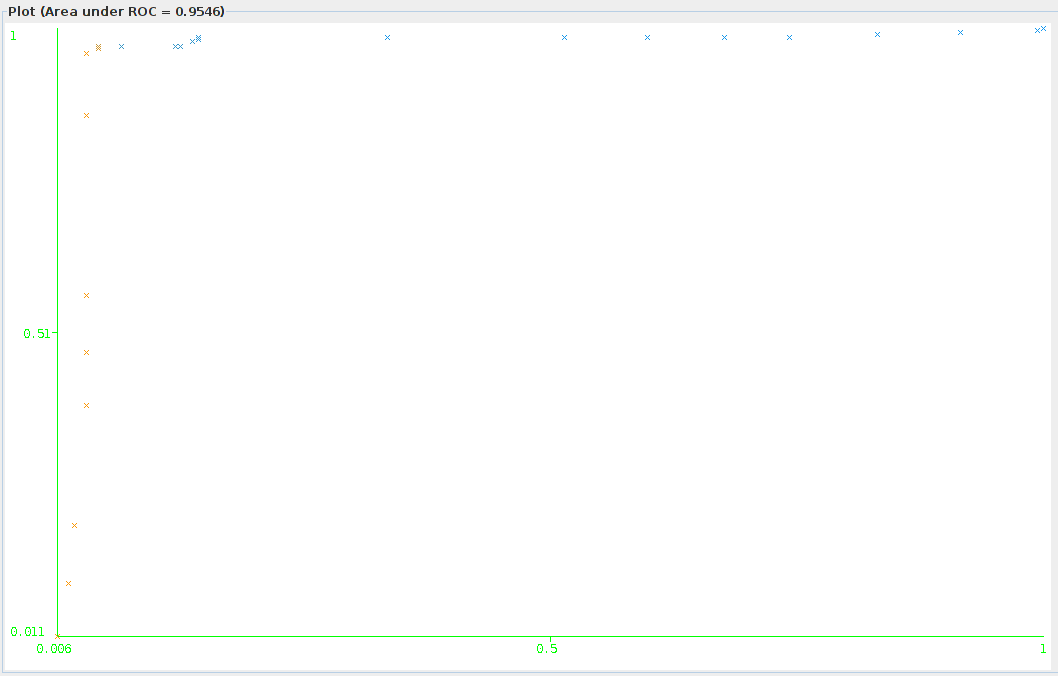
\includegraphics[height=5cm]{vote-j48-pruned}
            \caption{J48 (pruned) - ROC-Kurve für ``vote''}
        \end{figure}
    \end{frame}
    
    \begin{frame}[t]
    \frametitle{Aufgabe 4 - Entscheidungsbäume\\ ROC Kurven}
        Area Under ROC:
        \vfill
        \begin{tabular}[htbp]{l||c|c|c}
            Datensatz & ID3 & J48 (unpruned) & J48 (pruned) \\
            \hline
            \hline
            breast-cancer & 0.5368 & 0.5742 & 0.5823 \\
            \hline
            vote & 0.9363 & 0.9647 & 0.9546 \\
        \end{tabular}
        \vfill
	\begin{itemize}
            \item Der Datensatz \textit{breast-cancer} scheint  mit den verwendeten Klassifizieralgorithmen nicht gut lernbar zu sein
            \item J48 hat generell eine deutlich bessere Performance als ID3 
\begin{itemize}	    
\item Aber hier ist zumindest im Bezug auf die Area under ROC kein eindeutiger Unterschied bei Pruning erkennbar
        \end{itemize}
        \end{itemize}
    \end{frame}
    
    \subsection{Accuracy und Baumgröße}
    
    \begin{frame}[t]
    \frametitle{Aufgabe 4 - Entscheidungsbäume\\ Accuracy und Baumgröße}
        \begin{tabular}[htbp]{l||c|c|c}
            Datensatz & ID3 & J48 (unpruned) & J48 (pruned) \\
            \hline
            \hline
            \multirow{2}{*}{breast-cancer} & 57\% Accuracy & 68.5\% Accuracy & 75.5\% Accuracy \\
            & \textasciitilde 465 Knoten & \textasciitilde 180 Knoten & 6 Knoten \\
            \hline
            \multirow{2}{*}{vote} & 93\% Accuracy & 95\% Accuracy & 96\% Accuracy \\
            & \textasciitilde 60 Knoten & 25 Knoten & 6 Knoten \\
        \end{tabular}
        \vfill
        \begin{itemize}
            \item J48 erreicht eine höhere Genauigkeit als ID3\\
            \item Pruning erhöht die erzielte Genauigkeit weiter
\begin{itemize}
                \item Resultierender Baum generalisiert besser und vermeidet Overfitting
            \end{itemize}
            \item Die Bäume von ID3 sind viel größer als die von J48
\begin{itemize}
                \item Ziel von ID3: In jedem Blatt nur Beispiele einer einzigen Klasse 
            \end{itemize} 
            \item (Post-)Pruning bei J48 reduziert die Baumgröße deutlich
            \begin{itemize}
                \item Knoten entfernen, wenn dadurch der erwartete Fehler geringer wird
                \item Verhindern von Fragmentierung (Minimalanzahl an Instanzen in Knoten)
            \end{itemize}
        \end{itemize}
    \end{frame}
    
    \section{Aufgabe 5 - Nearest Neighbour}
    
    \subsection{Benutzte Datensätze}
    
    \begin{frame}[t]
    \frametitle{Aufgabe 5 - Nearest Neighbour\\ Benutzte Datensätze}
        \begin{itemize}
            \item Breast Cancer Data
            \item 1984 United States Congressional Voting Records Database
        \end{itemize}
        \vfill
        $\rightarrow$ Auf beide Datensätzen den unsupervised Filter ``ReplaceMissingValues'' anwenden 
        $\rightarrow$ Danach anwenden und evaluieren von IBk
    \end{frame}
    
    \subsection{Resultat}
    
    \begin{frame}[t]
    \frametitle{Aufgabe 5 - Nearest Neighbour\\ Resultat}
        Cross Validation Accuracy:
        \vfill
        \begin{tabular}[htbp]{l||c|c|c|c|c|c|c}
            Datensatz & k=1 & k=3 & k=5 & k=7 & k=9 & k=11 & Aufg. 4 \\
            \hline
            \hline
            breast-cancer & 71.7\% & 74.1\% & 73.8\% & 73.8\% & 73.8\% & 72.7\% & 75.5\% \\
            \hline
            vote & 93.6\% & 93.1\% & 94.0\% & 93.3\% & 92.9\% & 92.6\% & 96\% \\
        \end{tabular}
        \vfill
\begin{itemize}
       \item Es gibt keinen allgemeinen besten Wert für k
\begin{itemize}
\item Dieser muss experimentell festgestellt werden
\end{itemize}
        \item  Bei beiden Datensätzen führen zu kleine und zu große Werte für k zu einer schlechteren Genauigkeit (Noise bzw. zu große Neighborhood)\\
\end{itemize}
    \end{frame}
    
    \section{Aufgabe 6 - Regressionsbäume}
    
    \subsection{Benutzte Datensätze}
    
    \begin{frame}[t]
    \frametitle{Aufgabe 6 - Regressionsbäume\\ Benutzte Datensätze}
        \begin{itemize}
            \item Auto Price Dataset
            \item Concrete Compressive Strength
            \item Boston Housing Data
            \item Stock Prices Dataset
            \item Wine Quality
        \end{itemize}
        \vfill
        $\rightarrow$ Benutzen von M5P mit verschiedenen Optionen
    \end{frame}
    
    \subsection{Pruning}
    
    \begin{frame}[t]
    \frametitle{Aufgabe 6 - Regressionsbäume\\ Pruning}
        \begin{tabular}[htbp]{l||c|c}
            Datensatz & Unpruned & Pruned \\
            \hline
            \hline
            \multirow{2}{*}{autoprice} & MAE 2075, RMSE 3287 & MAE 2096, RMSE 3336 \\
            & Number of Rules 62 & Number of Rules 8 \\
            \hline
            \multirow{2}{*}{concrete} & MAE 6.5, RMSE 8.3 & MAE 6.9, RMSE 8.7 \\
            & Number of Rules 405 & Number of Rules 60 \\
            \hline
            \multirow{2}{*}{housing} & MAE 3.2, RMSE 4.7 & MAE 3.3, RMSE 4.8 \\
            & Number of Rules 193 & Number of Rules 26 \\
            \hline
            \multirow{2}{*}{stock} & MAE 1.2, RMSE 1.6 & MAE 1.2, RMSE 1.6 \\
            & Number of Rules 253 & Number of Rules 88 \\
            \hline
            \multirow{2}{*}{winequality} & MAE 0.5, RMSE 0.7 & MAE 0.6, RMSE 0.7 \\
            & Number of Rules 1562 & Number of Rules 73 \\
        \end{tabular}
        \vfill
\begin{itemize}
       \item Pruning verringert die Größe des Baumes deutlich, während der Fehler nur geringfügig größer wird
        \item Bei Regression Trees ist Pruning sinnvoll, um fast ohne Performanceverlust die Interpretierbarkeit zu erhöhen
\end{itemize}
    \end{frame}
    
    \subsection{Model Trees}
    
    \begin{frame}[t]
    \frametitle{Aufgabe 6 - Regressionsbäume\\ Model Trees}
        \begin{tabular}[htbp]{l||c|c}
            Datensatz & Pruned & Model Tree \\
            \hline
            \hline
            \multirow{2}{*}{autoprice} & MAE 2096, RMSE 3336 & MAE 1467, RMSE 2171 \\
            & Number of Rules 8 & Number of Rules 10\\
            \hline
            \multirow{2}{*}{concrete} & MAE 6.9, RMSE 8.7 & MAE 4.7, RMSE 6.4 \\
            & Number of Rules 60 & Number of Rules 10 \\
            \hline
            \multirow{2}{*}{housing} & MAE 3.3, RMSE 4.8 & MAE 2.5, RMSE 3.8 \\
            & Number of Rules 26 & Number of Rules 19 \\
            \hline
            \multirow{2}{*}{stock} & MAE 1.2, RMSE 1.6 & MAE 0.7, RMSE 0.9 \\
            & Number of Rules 88 & Number of Rules 47 \\
            \hline
            \multirow{2}{*}{winequality} & MAE 0.6, RMSE 0.7 & MAE 0.5, RMSE 0.7 \\
            & Number of Rules 73 & Number of Rules 24\\
        \end{tabular}
        \vfill
\begin{itemize}
        \item Model Trees scheinen noch besser zu sein
\begin{itemize}
\item fast immer kleiner und zusätzlich weisen sie kleineren Fehler auf
\end{itemize}
        \item Ursache könnte umfassendere Betrachtung der einzelnen Attribute im linearen Modell sein, anstatt nur den Mittelwert der Instanzen zu verwenden
\end{itemize}
    \end{frame}
    
\begin{frame}
\frametitle{Abschlussüberblick}
\tableofcontents
\begin{center}
\end{center}
\end{frame}

\begin{frame}
\frametitle{Gruppenmitglieder}
Joachim Brehmer, 1766932  \vfill
Jeannine Endreß, 1669152 \vfill
Uli Fahrer, 1664571
\end{frame}

\end{document}
